\chapter[Processo de Desenvolvimento de Software]{Processo de Desenvolvimento de Software}
\label{cp:processo_de_desenvolvimento}

Como definido o tópico \ref{sec:processo_de_desenvolvimento_de_software}, o processo de desenvolvimento de \textit{software} deste projeto pode ser visualizado na Figura \ref{img:processo_de_desenvolvimento}. A descrição das atividades do processo serão definididas a seguir: 

\begin{figure}[H]
	\centering
	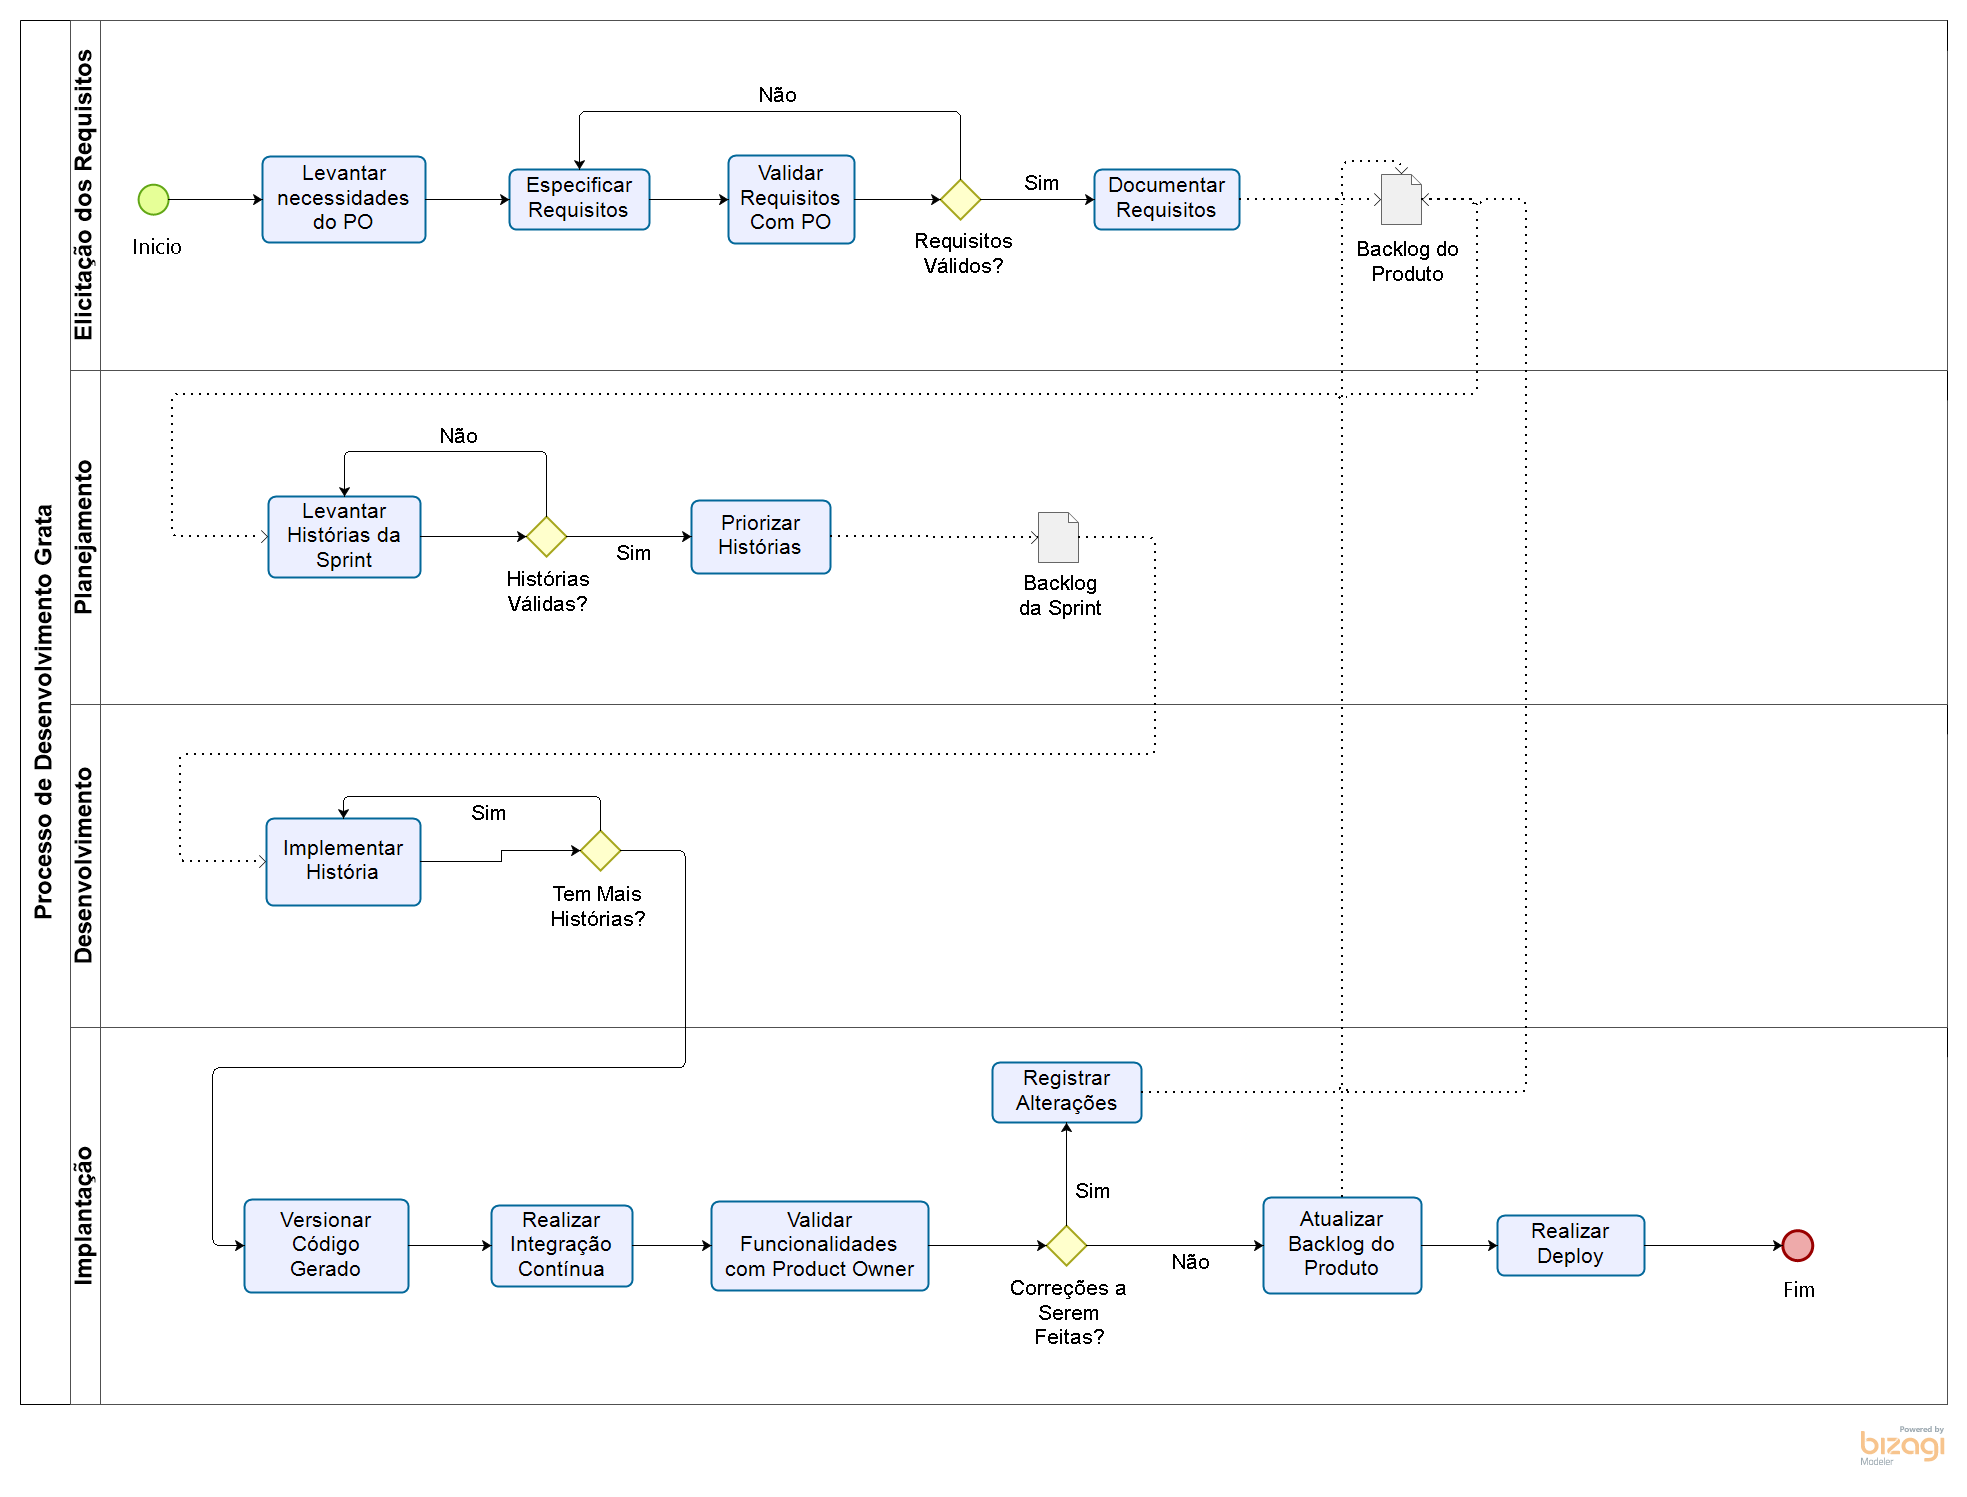
\includegraphics[width=1.0\textwidth]{figuras/processo_de_desenvolvimento.png}
	\caption{Processo de Desenvolvimento do Grata}
	\label{img:processo_de_desenvolvimento}
\end{figure}



% FRONT-END
% A linguagem \textit{front-end} escolhida para este projeto, foi o \textit{React}, pois além de facilitar o desenvolvimento e interação com usuário final, é uma das mais utilizadas ao redor do mundo, então facilita uma manutenção futura e evolução do \textit{software}.


% BACK-END
% A linguagem \textit{back-end} escolhida para este projeto, foi a \textit{Python Django-Rest}, pois tem uma ótima conexão com a linguagem \textit{front-end}, e por ser muito utilizada, possibilitando assim uma manutenção e evolução futura.

%  Neste projeto a arquitetura adotada é uma adaptação ao padrão arquitetural MVC \textit{(model-view-controller)}.



% \subsubsection{Arquitetura do Projeto}

% Neste projeto é feita uma adaptação ao padrão MVC, por conta da escolha da linguagem \textit{front-end}. O \textit{React} possui um padrão arquitetural diferente, chamado de arquitetura de componentes/microserviços. Esse padrão possui semelhanças ao MVC, e o que será utilizado dele será a parte da \textit{View}. Enquanto a linguagem \textit{back-end} é responsável por trabalhar os dados provindos do \textit{front-end} e oferecer um retorno a ele. 

A seguir será mostrado como funciona separadamente o \textit{React},relacionado ao \textit{front-end} que engloba a \textit{View}, enquanto o \textit{Python Django-Rest} é responsável pelo \textit{back-end} e que engloba a \textit{Model} e a \textit{Controller}:

\begin{figure}[H]
	\centering
	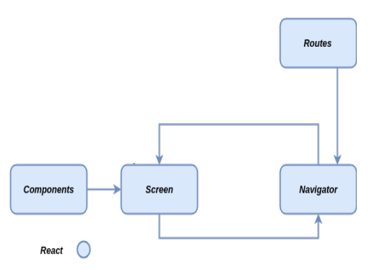
\includegraphics[width=1.0\textwidth]{figuras/diagrama_react.png}
	\caption{Diagrama React/Microsserviços}
	\label{img:diagrama_react}
\end{figure}

\begin{figure}[H]
	\centering
	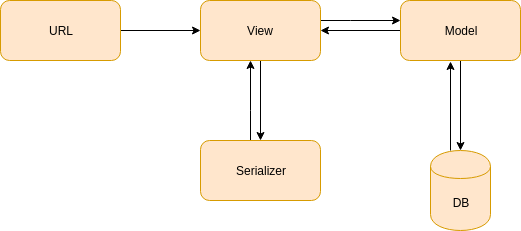
\includegraphics[width=1.0\textwidth]{figuras/django_rest.png}
	\caption{Diagrama Django REST Framework}
	\label{img:diagrama_rest}
\end{figure}

\section{Cronograma TCC}
